% macros for comments
\newcommand{\maren}[1]{{\color{cyan} \textbf{[Maren: #1]}}}
\newcommand{\andrei}[1]{{\color{red} \textbf{[Andrei: #1]}}}

\section{Introduction}\label{introduction}

Data selection is a major challenge in supervised machine learning (ML). Quite often when data is abundant, it is collected prior to the training process and provided statically, meaning that the machine learning model has no influence on the data collection process. However, if data is expensive and scarce the performance of a model trained on a static dataset can be suboptimal or even poor. In those cases, it is beneficial to carefully select the dataset such that, for example, it is maximally informative under the ML model to achieve the task at hand. This branch of ML is generally referred to as \emph{active learning} \cite{Settles2009} and has attracted attention in various sub-fields such as \emph{experimental design} (the task of predicting an unknown function value from its input), \emph{global optimisation} (guessing the global minimiser of a function) and \emph{integration} (guessing the integral of a function).
The Emukit Python library, at core, augments existing machine learning models with active data selection functionality.

Tasks where data is scarce usually involve a higher degree of expert knowledge on the modeling side since prior information, such as mechanical or physical knowledge about the system that is being modeled, is aimed to be incorporated in the hope to get physically meaningful and more accurate predictions on the task at hand. Not seldom these models are of probabilistic nature and can provide a degree of uncertainty of their prediction to counteract the lack of data \cite{RasmussenWilliams2006, Ho1995, MacKay1991APB, Smith1998UncertaintyAA}. Such a model is often referred to as a \emph{statistical emulator}\footnote{The reader might be familiar with the term `emulator' in computing context, where it is understood as a hardware or software that makes one system behave like another. `(Statistical) emulator' we refer to throughout this paper is an unrelated, albeit similar, term from the machine learning literature.}, which is a machine learning model that can be used in place of an expensive computer simulation (a \emph{simulator}) or real world experiment, and is trained on input-output pairs of the latter. \cite{Kennedy2000, Kennedy2001, Conti2009, Conti2010}. Concretely, the simulator could be an involved stochastic weather simulation, and the emulator a predictive machine learning model trained on expensive input-output pairs of the weather simulation. Alternatively, the emulator may model a real world process. The emulator now can be used in place of the original data source to obtain fast predictions when needed, or to compute auxiliary quantities that cannot be obtained from the data source.

Once trained, the performance of the emulator (the ML model), as mentioned, is greatly dependent on the informativity of the data (the simulation results), especially if it is expensive and scarce, and hence active data selection is often desirable for such models. A unique feature of Emukit is that it enables the user to wrap custom emulator models into an interface provided by Emukit and, by doing so, use them in Emukit's decision loop. As such, Emukit `actifies' (makes active) the data-acquisition of custom models written in custom backends that only connect via an interface to Emukit. This may i)~save users time and money to write their own active learning loop, ii)~or to rewrite their custom model in existing decision loop packages with a fixed backend, and iii)~improve performance of the model as it is trained on more informative data.

Hence, the most prominent features of Emukit can be summarized as follows.

\begin{itemize}
\item Emukit \emph{augments existing models with active learning} capability, in particular models used in Bayesian optimisation, Bayesian quadrature and experimental design.
\item Emukit can use existing, potentially specialized, custom models provided by the user and wrap them into a provided interface. As such Emukit is \emph{model backend agnostic}.
\item Emukit is highly abstracted and mimics the components of an active decision loop. This composability allows users to provide custom implementations of subroutines and classes that seamlessly integrate with the rest of the package. Hence Emukit is \emph{highly flexible} and allows \emph{fast and easy prototyping}.
\item In contrast to other packages, Emukit provides several active learning methods via \emph{subpackages that share a core implementation of the active learning loop}. This enables the user to potentially use the same model backend and even the same model instance across tasks. This increases consistency between results, may reduce implementation overhead and my allows resource sharing between tasks.
\item Emukit provides basic functionality for \emph{multi-fidelity modeling} which allows the user to incorporate data sources of different fidelities. Further, Emukit contains a limited number of model wrappers to illustrate their usage and some example applications.
\end{itemize}

The remainder of the paper corroborates on the points above in greater detail. The following section briefly introduces the supported machine learning methods before Emukit's workflow and library structure is sketched.
%and Section~\ref{} exemplifies usage. Sections~\ref{} and \ref{} discuss related libraries and limitations of Emukit respectively.
Throughout the text, `tasks' will be referred to in an abstract sense, without a specific application in mind.
%This is because Emukit is abstracted away from a specific application and can be used for a variety of tasks that obey a certain algorithmic structure (more in this in Section~\ref{}.
In the remainder of text, we will use the terms `ML model' and `emulator' interchangeably. The `simulator' or `data source' will later also be referred to as `user function', `black-box function' or `objective function'.

\section{Background on probabilistic active methods}\label{sec:background}

This section gives an overview of the machine learning methods provided by Emukit.
Emukit mainly contains three high-level methods: Bayesian optimisation (BO), Bayesian quadrature (BQ) and experimental design (ED).

\emph{Bayesian optimisation} \cite{Mockus1978, Garnett2023} is a numerical method that aims to guess the global minimiser of a black-box function by querying function values at nodes and returning the minimiser of the collected set. Corresponding algorithms are inherently sequential and, at every iteration, decide on where to query the objective function next. The decision solves the so called `exploration-exploitation trade-off' between exploring unknown regions of the function's domain, or exploiting rather promising regions of a potential minimiser. This trade-off is encoded in a heuristic called `acquisition function' that quantifies the usefulness of evaluating the function at a certain node. Hence, BO is generally sample-efficient and thus especially useful when the function is expensive to evaluate and the number of allowed evaluations is limited. There exists a large range of heuristics and methods that all fall under the umbrella of BO, out of which Emukit supports several. Bayesian optimisation has been successfully applied in various fields \cite{baheri2017altitude, graff2021accelerating}, but most notably in the automation of hyperparameter tuning tasks of neural networks \cite{snoek2012practical, avent2020automatic}.

\emph{Bayesian quadrature} \cite{Diaconis1988, OHagan1992, pnbook22} is a numerical method that aims to infer the integral of a black-box function (called the `integrand') given some integration measure and queries of the integrand at nodes. In contrast to Monte Carlo (MC) methods, BQ generally can accept any kind of node design and is especially sample efficient which makes it superior to MC in certain circumstances \cite{RasmussenGhahramani2002}. A sub-group of BQ methods are active and follow a similar decision loop as BO; the most notable difference being that acquisition functions are specific to BQ and the class of models is somewhat more restricted. Generally, active BQ methods are algorithmically similar on a high level to BO methods and can use similar models.

\emph{Experimental design} \cite{Kennedy2000, Kennedy2001, Conti2009, Conti2010} is a method that aims to collect nodes of a black-box function such that the resulting model predicts unseen function values well. It has traditionally been applied to statistical emulation of complex computer models \maren{cite} but also to \maren{examples?}. Some ED methods, too, obey the structure of an active decision loop similar to BO and BQ.

Emukit is build on the realization that all three methods (BO, BQ, ED), albeit having different numerical aims and result objects, share the same algorithmic structure: a decision loop that computes the next node based on the current model, evaluates the user function and then updates the model accordingly. This decision loop is contained in Emukit's core package and shared by all three high-level methods.
%Thus Emukit contains are shared core implementation of the decision loop of all three methods which will be elaborated further on in Section~\ref{sec:lib-structure}.
Further, especially BO and ED can use similar models while BQ is somewhat more restricted. Potential benefits of shared implementation, model and compute among tasks are discussed in later sections.

Finally, Emukit provides basic support of \emph{multi-fidelity models} \cite{Peherstorfer2017} which can combine query results of the black-box function of different quality (from low fidelity to high fidelity). This yields multi-fidelity BO, BQ and ED methods that can be made active again with Emukit's decision loop.


\section{Emukit workflow}\label{sec:workflow}
Decision making with statistical emulation consists of three parts. All starts with a \textit{task}, a high level goal that we are interested in achieving. It usually involves a complex process that we aim to study and answer a question about. Some examples include finding the best operation mode of a drone, measuring the quality of a weather simulation, explaining behavior of a complex system. In order to solve the task we choose a \textit{method}, a relatively low-level technique that guides our exploration of the target process and provides the quantifiable way to answer the task's question. Examples include Bayesian optimisation, Bayesian quadrature and experimental design. And finally there is a \textit{model}, a probabilistic data-driven representation of the process under study. Examples of such models are a Gaussian process, a random forest or a Bayesian network. Consequently, the typical workflow for users working with Emukit consists of three steps (see Figure~\ref{figure:workflow} for a graphical description).

\textbf{Build the model.} Instead of constraining the user to certain model classes, Emukit provides the flexibility of using user-specified models. Generally speaking, Emukit does not provide modelling capabilities. Instead users are expected to define their own models. Because of the variety of modelling frameworks available, Emukit does not mandate or make any assumptions about a particular modelling technique or a library, and suggests to implement a subset of defined model interfaces that are required to use a particular method.

\textbf{Run the method.} This is the main focus of Emukit. Emukit defines a general structure of a decision making method and offers implementations of several such methods: Bayesian optimisation, Bayesian quadrature, experimental design. All methods are model-agnostic and only rely on model interfaces.

\textbf{Solve the task.} For the end users, Emukit is a way to solve a certain task, which may have research or business value. Emukit provides a set of examples of how tasks such as hyperparameter tuning, sensitivity analysis, multi-fidelity modelling or benchmarking are accomplished using the library.

\begin{figure}[h]
    \centering
    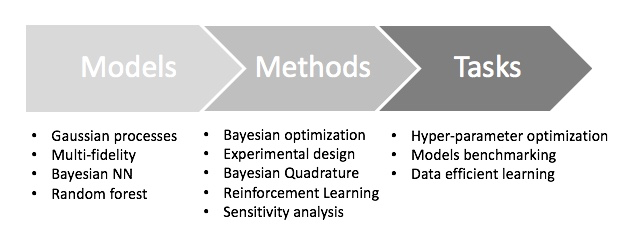
\includegraphics[scale=0.4]{workflow.png}  
    \caption{Summary of workflow for the users of Emukit. A model is computed in a modelling framework of choice. The model is wrapped using a pre-defined interface and connected to the core components of several methods such as Bayesian optimisation, experimental design etc. Specific tasks are then solved using these methods.}
    \label{figure:workflow}
\end{figure}

\section{Structure of the library}\label{sec:lib-structure}

At a conceptual level the methods supported in Emukit -- such as Bayesian optimisation, experimental design and Bayesian quadrature -- are all iterative decision making processes that follow a similar pattern. Algorithmically they can be thought of as instances of a common abstract loop, which we now describe (also see Algorithm~\ref{alg:emukit-loop}).

The common goal of all these methods is to learn a behavior of an \textit{objective function} - a black box expensive process that has certain \textit{parameters}. The knowledge about the objective function (initially available as well as that collected during the learning process) is represented with a \textit{probabilistic model}. A mechanism employed to propose new data points to evaluate the objective at is called a \emph{policy} that maximises an \textit{acquisition function}. Finally, the decision making process is done in a \textit{loop} until a certain \textit{stopping condition} is met. 

\begin{algorithm}[H]
  \caption{Decision making loop in Emukit.}
  \label{alg:emukit-loop}
  \begin{algorithmic}[1]
    \While{stopping condition is not met}
      \State collect next point(s) for evaluation
      \State evaluate objective function
      \State update model with new observation(s)
    \EndWhile
  \end{algorithmic}
\end{algorithm}

The internal structure of Emukit reflects these abstractions to ensure that fundamental components of the decision making loop could be swapped out and replaced. While some of the basic components in Emukit correspond to the parts of the decision making loop exactly, others are more fine-grained to allow for greater flexibility and plug-and-play experience for the researchers using the package. We will now give an overview of these components.

\textbf{Outer Loop}. The \texttt{OuterLoop} class is the abstract loop where the different components come together. Loops for specific methods, such as Bayesian optimisation and experiment design, should subclass it. The library provides several concrete implementations of the loop, and also contains examples how the users can build their own.

\textbf{Parameter space}. Represents the parameter space of the objective function, also referred to as input space. Emukit supports continuous, categorical, discrete, and bandit parameters.

\textbf{Model}. All Emukit loops need a probabilistic model. Emukit does not provide functionality to build models as there are already good modelling frameworks available in Python. Instead, it provides a way of interfacing third part modelling libraries. The interfacing mechanism consists of two parts: interfaces and wrappers. \textit{Interfaces} define functionality required from a model. Different models and modelling frameworks will provide different functionality. For instance a Gaussian process will usually have derivatives of the predictions available but random forests will not. These different functionalities are represented by a set of interfaces which a model implements. The basic interface that all models must implement is \texttt{IModel}, which implements functionality to make predictions and update the model but a model may implement any number of other interfaces such as \texttt{IDifferentiable} which indicates a model has prediction derivatives available. Interfaces can also be defined by other components of the decision making loop to indicate that a certain functionality is required from the model. For example, \texttt{ICalculateVarianceReduction} defines methods the user needs to implement with their model to use it with the variance reduction technique. \texttt{Model wrappers} adopt third-party models and implement one or more of the interfaces using specific modelling framework. Emukit provides a wrapper for using a model created with \texttt{GPy} \cite{gpy2014}.

\textbf{Candidate Point Calculator}. This entity drives the decision on which point(s) to evaluate next. The simplest implementation provided out of the box, \texttt{SequentialPointCalculator}, collects one point at a time by finding where the acquisition is at a maximum by applying the acquisition optimiser to the acquisition function. More complex implementations are possible, for example to enable batches of points to be collected so that the user function can be evaluated in parallel.

\textbf{Acquisition}. The acquisition is a function defined on the parameter space that produces continuous values. It represents a heuristic quantification of how valuable collecting a future point might be, and produces continuous values. It is used by the candidate point calculator to decide which point(s) to collect next. Acquisition functions balance exploration and explotation of the decision making process.

\textbf{Acquisition Optimiser}. The \texttt{AcquisitionOptimizer} optimises the acquisition function to find the point at which the acquisition is at a maximum. If available, the optimiser can use the acquisition function gradients. Otherwise, it will either estimate the gradients numerically, or use a gradient free optimisation.

\textbf{User Function}. This is the component that represents the objective function. It can be evaluated by the user, or it can be passed into the loop and evaluated by Emukit.

\textbf{Model Updater}. The \texttt{ModelUpdater} class updates the model with new training data after a new point is observed and optimises any hyper-parameters of the model. It can decide whether hyper-parameters need updating based on some internal logic.

\textbf{Stopping Condition}. The \texttt{StoppingCondition} class chooses when the decision making loop should stop collecting points. The most commonly used approach is to stop when a set number of iterations has been reached.

These are the core components Emukit defines. Specific methods can also define additional concepts of their own, e.g. integration measures or costs. Table~\ref{table:abstraction_mapping} shows the mapping between decision making abstractions and Emukit components.

\begin{table}
    \setlength{\DUtablewidth}{\tablewidth}
    \begin{longtable}[c]{p{0.4\DUtablewidth}p{0.4\DUtablewidth}}
        \toprule
        \textbf{Decision making abstractions} & \textbf{Emukit components} \\
        \midrule
        \endfirsthead
        Loop & Outer loop \\
        \midrule
        Parameters & Parameter space \\
        Probabilistic model & Model interface \\
        & Model wrapper \\
        \midrule
        Acquisition function & Candidate point calculator \\
        & Acquisition \\
        & Acquisition optimiser \\
        \midrule
        Objective function & User function \\
        & Model updater \\
        \midrule
        Stopping Condition & Stopping condition \\
        \bottomrule
    \end{longtable}
    \caption{The mapping between abstractions of the decision making process and the components defined in Emukit.}
    \label{table:abstraction_mapping}
\end{table}

\section{Usage overview}\label{sec:usage}
This section describes Emukit's high level APIs for all main functions of the package: Bayesian optimisation, Bayesian quadrature, experimental design and multi-fidelity emulation. Unless stated otherwise, we assume that some initial data (an initial design of reasonable size with corresponding evaluations of the user function) is already defined and stored in the variables \texttt{X} (inputs) and \texttt{Y} (values). We use GPy \cite{gpy2014} in the code snippets below for modelling, and exclude import lines for brevity.

\subsection{Standard methods and models wrapping}

Interfaces for Bayesian optimisation and experimental design are the most straighforward ways to use the library. Both methods require the user to define a model and wrap it in the Emukit's model wrapper. An input space also has to be defined using Emukit's classes. The choice of acquisition function is optional, as reasonable defaults are provided. High level loop objects allow the user to execute the decision making loop and access its properties.

\begin{verbatim}
model_gpy = GPy.models.GPRegression(X,Y)
model_emukit = GPyModelWrapper(model_gpy)

parameter_space = ParameterSpace([
    ContinuousParameter('x1', -5, 10),
    ContinuousParameter('x2', 0, 15)
])

expected_improvement_acquisition =
    ExpectedImprovement(model = model_emukit)
bayesopt_loop = BayesianOptimizationLoop(
    model = model_emukit,
    space = parameter_space,
    acquisition = expected_improvement_acquisition
)

model_variance_acquisition =
    ModelVariance(model = model_emukit)
experimental_design_loop =
    ExperimentalDesignLoop(
        model = model_emukit,
        space = parameter_space,
        acquisition = model_variance_acquisition
    )
\end{verbatim}

Usage of Bayesian quadrature (BQ) API is more envolved, as even in its most basic form it requires more choices from the user. First the objective function, also referred to as an integrand, is modelled with a Gaussian process (GP). Since BQ integrates the kernel function, the kernel is then wrapped in a separate Emukit object. Bundled together, wrappers around the kernel and the model itself represent a base model in the BQ package. This model can be used with several BQ methods, the code below illustrates vanilla Bayesian quadrature where the GP model is directly placed over the integrand function and then integrated analytically.

\begin{verbatim}
lb = -3.0 # lower integral bound
ub = 3.0 # upper integral bound
gpy_model = GPy.models.GPRegression(X=X, Y=Y)

emukit_rbf = RBFGPy(gpy_model.kern)
emukit_measure = LebesgueMeasure.from_bounds(
    bounds=[(lb, ub)]
)
emukit_qrbf = QuadratureRBFLebesgueMeasure(
    emukit_rbf, emukit_measure
)
gp_model = BaseGaussianProcessGPy(
    kern=emukit_qrbf, gpy_model=gpy_model
)

emukit_model = VanillaBayesianQuadrature(
    base_gp=gp_model, X=X, Y=Y
)
bq_loop = VanillaBayesianQuadratureLoop(
    model=emukit_model
)
\end{verbatim}

Once the loop object is created, either for optimisation, quadrature or experiment design, it can be evaluated in one of two modes. If the user has access to the objective function via Python, the loop can be managed by Emukit with the \texttt{run\_loop} method that accepts two arguments: the objective function and the stopping criterion. If the objective has to be called externally (e.g. a lab experiment has to be done), Emukit provides \texttt{get\_next\_points} method that produces the next evaluation point(s) based on the data observed so far. In that latter case user has to manage the decision making loop themselves.

\subsection{Interfaces for fast prototyping}
Emukit gives researchers a lot of flexibility in swapping individual pieces in and out of the decision making loop. This is made possible by clearly defined interfaces. We illustrate how this is accomplished in the package with an example of \texttt{IntegratedHyperParameterAcquisition}. This class provides an ability to integrate any acquisition function over hyperparameters of the model. To do that, the model needs to support two operations: generate hyperparameter samples and fix hyperparameters to a certain sample value. Consequently, Emukit defines an interface \texttt{IPriorHyperparameters} that declares these operations, and \texttt{IntegratedHyperParameterAcquisition} requires input model to implement this interfaces, as can be seen in the following code snippet:

\begin{verbatim}
class IPriorHyperparameters:
    def generate_hyperparameters_samples(...

    def fix_model_hyperparameters(...


class IntegratedHyperParameterAcquisition(Acquisition):
    def __init__(
        self,
        model: Union[IModel, IPriorHyperparameters],
        ...
\end{verbatim}

\subsection{Model reuse across tasks}

Emukit's composability allows to reuse components between methods. For example, we can use the quadrature model defined above to perform an optimisation loop, and then integrate it using the quadrature API. The ability to reuse components in this way lowers implementation overhead, optimises utilisation of compute resources, and increases consistency.

\begin{verbatim}
# see BQ snippet for complete
# definition of the model
emukit_bq_model = VanillaBayesianQuadrature(
    base_gp=gp_model, X=X, Y=Y
)

bayesopt_loop = BayesianOptimizationLoop(
    model = emukit_bq_model, space = parameter_space
)
n_iterations = 20
bayesopt_loop.run_loop(
    user_function,
    stopping_condition=n_iterations
)

emukit_bq_model.integrate()
\end{verbatim}


\subsection{Multi-fidelity emulation}

To support research on multi-fidelity emulation methods, Emukit implements both linear and non-linear multi-fidelity models. The user is expected to provide data for each of the fidelities and make the choice of appropriate Gaussian process kernel. Emukit can then be used to define a combined multi-fidelity model. In the example below we define a linear multi-fidelity model, where the relationship between fidelities is linear.

\begin{verbatim}
# This utility method allows to
# convert data from different fidelities
# to arrays where fidelity is represented
# as an input variable
X, Y = convert_xy_lists_to_arrays(
    [x_low, x_high],
    [y_low, y_high]
)

kernels = [
    GPy.kern.RBF(dim=1),
    GPy.kern.RBF(dim=1)
]
linear_mf_kernel =
    LinearMultiFidelityKernel(kernels)
gpy_linear_mf_model =
    GPyLinearMultiFidelityModel(
        X, Y,
        linear_mf_kernel,
        n_fidelities = 2
)
\end{verbatim}

\subsection{Other methods and features}
In addition to the APIs discussed above, Emukit also provides basic support for sensitivity analysis and benchmarking. Further information about Emukit's functionality, including available implementations of acquisition functions, multi-output models, support for constraints and cost functions, custom events in the outer loop, can be found in library's website\footnote{\url{https://emukit.github.io/}}, documentation\footnote{\url{https://emukit.readthedocs.io/en/latest/}} and tutorial notebooks\footnote{\url{https://nbviewer.org/github/emukit/emukit/blob/main/notebooks/index.ipynb}}. 

\section{Emukit in action}
Since its announcement in 2019 \cite{paleyes2019emulation}, Emukit was used in a wide range of research projects. In this section we review a selection of these projects to showcase the breadth of situations in which the library can be useful.

\subsection{Methodological research}
Because of its flexibility Emukit allows researchers to rapidly experiment with decision making methods in its suite. In this section we discuss several research papers that leverage this fact to advance the field of decision making under uncertainty.

Optimisation of parameters in high dimensional structured data spaces is an increasingly important and challenging task. A common pattern is to use unsupervised learning methods to project parameters into low dimensional continuous representations, also known as latent spaces. There are multiple ways to approach the design of the Bayesian optimisation procedure on such latent spaces. Siivola et al. \cite{siivola2021good} study the effects of various design choices. Namely, the effects of the dimensionality of the latent space, the optimisation bounds, and the choice of acquisition function are analysed. Emukit's plug-and-play approach allowed the researchers to facilitate measurement of these effects in isolation.

Emukit's composability was also leveraged for the implementation of BOSH, a sampling approach for Bayesian optimisation of functions with stochastic evaluations \cite{moss2020bosh}. Authors used hierarchical Gaussian process as a surrogate and designed a novel BOSH acquisition function using the information-theoretic framework, incorporating both pieces in Emukit's Bayesian optimisation loop. Emukit was also used to assess BOSH performance against a variety of baselines.

Naslidnyk et al. \cite{Naslidnyk21} implemented a custom Bayesian quadrature model and used Emukit's existing BQ wrapper and decision loop in order to learn integrals of functions that are input invariant under some transformations. They tested their method on a problem from Fourier optics where the integral over a point spread functions of symmetric lenses was computed. Further, Gessner et al. \cite{Gessner20} applied Emukit in the context of active multi-source Bayesian quadrature. The authors implemented a custom multi-source BQ model, a corresponding wrapper and even a custom multi-source acquisition function and point calculator which was possible due to Emukit's abstraction and plug-and-play capability.

\subsection{Example applications}
In this section we describe several cases where Emukit was used to solve a problem in other scientific domains.

Bell et al. used Emukit to show how to conduct multiverse analysis for machine learning experiments \cite{bell2022modeling}. Multiverse analysis was originally introduced in psychology, and allows researchers to explore the robustness and generality of claims by systematically examining the impact of different choices and variations in the experimental setup. The authors argue that the same concept can be applied to the machine learning: if a new technique, e.g. batch normalization, is proposed for an ML model, it should remain effective regardless of the model architecture, optimisation method, dataset, evaluation metric, and so on. The set of these variations comprises a multiverse, and needs to be explored effectively. The authors use surrogate modelling and Bayesian experimental design to systematically explore the effect of each choice. Emukit was chosen as an implementation tool because of the experimental design API it provides.

Uhrenholt and Jensen used Emukit's Bayesian optimisation module to solve the problem of finding settings of a musical synthesizer to produce a given sound \cite{uhrenholt2019efficient}. A musical synthesizer produces sound by generating waveforms via oscillators. Created audio streams are then routed through a pipeline that consists (not necessary all) of mixing of separate streams, filtering, adding of noise, and saturation. Musicians can control the output sound by changing the configuration of the pipeline. In order to estimate the discrepancy between the produced sound and the target, the authors designed a novel modeling approach, in which Gaussian process is used to model the distribution of the output's L2 norm. The flexibility of Emukit allowed to implement this customization directly, without necessary effort duplication. Emukit's API also facilitated a fair comparison to standard Bayesian optimisation baseline.

Liyanage et al. faced the problem of combining data from multiple particle accelerators, including Large Hadron Collider and Relativistic Heavy Ion Collider, to study the properties of quark-gluon plasma \cite{PhysRevC105034910}. Nuclear collision experiments generate a large body of measurements with varying levels of uncertainty that would be expensive to quantify with simulations. Instead the authors proposed to use inexpensive statistical emulators and use transfer learning to leverage similarities between different heavy ion collisions systems. This new technique is based on multi-fidelity emulation, making Emukit an obvious implementation choice.

\section{Related work}
The Python ecosystem is rich with powerful scientific packages, including those for decision making methods.

In particular, \emph{Bayesian optimisation} enjoys a wide selection of tools and frameworks. Spearmint \cite{snoek2012practical} and GPyOpt \cite{gpyopt2016} are among the first Python packages for Bayesian optimisation, the latter being an inspiration for the first release of Emukit. BoTorch \cite{balandat2020botorch} is a popular library for Bayesian optimisation based on PyTorch. Similarly, Trieste \cite{picheny2023trieste} also focuses on Bayesian optimisation but uses Tensorflow as a backend. More options, such as pyGPGO \cite{jimenez2017pygpgo}, scikit-optimize \cite{louppe2017bayesian}, RoBO \cite{klein-bayesopt17}, are also available.

For \emph{Bayesian quadrature} and \emph{Bayesian experimental design} the choice of frameworks is more scarce. Namely, bayesquad \cite{Charles2013} appears to be another Python package for Bayesian quadrature. The Python library ProbNum \cite{Wenger21} supports a variety of Bayesian quadrature methods, but it's lack of hyper-parameter tuning capability reduces its practical relevance significantly in its current form. Optbayesexpt \cite{mcmichael2021optbayesexpt} and NEXTorch \cite{wang2021nextorch} provide Bayesian experimental design functionality adopted for their respective fields. Elements of experimental design can also be found in Trieste \cite{picheny2023trieste}.

The key difference between Emukit and the mentioned libraries is the fact that Emukit does not dictate a particular modelling framework, allowing for flexibility in the choice of computational backends. In addition, Emukit does not focus on a single method and provides a common core set of abstractions for optimisation, quadrature and experimental design. Emukit provides a unique way of using the same model backend for all tasks, which increases consistency, reduces implementation and computing overheads.

Likewise, we were not able to locate a Python library other than Emukit that provides multi-fidelity emulation functionality. A notable package for research on multi-fidelity methods is MF2 \cite{vanRijn2020} that implements a variety of multi-fidelity benchmark functions, but does not have modelling capabilities.

Looking at a wider family of optimisation libraries in Python, Optuna \cite{optuna_2019} is a popular choice for hyperparameter optimisation. Similarly to Emukit, Optuna is framework agnostic, however it provides a different set of optimisation methods, focusing on evolutionary, genetic and Monte Carlo based approaches. Finally, Ray Tune \cite{liaw2018tune} is a well known scalable platform in Python on which other model optimisation frameworks can be executed. Emukit can potentially be integrated with Ray Tune as an optimisation library. This work was not carried out yet, and can be a future development direction.

\section{Limitations}\label{section:limitations}
The design choices made in Emukit have proven to be highly beneficial for rapid prototyping and experimentation. However they also led to some of the key limitations of the library.

Emukit does not provide modelling capabilities, and instead requires users to provide their own surrogate models. This requires certain level of proficiency with probabilistic modelling, and can prevent some people from using the library. While we aim to mitigate this with extensive collection of examples and tutorials, and Emukit is successfully used in teaching university-level courses and scientific summer schools, the library still cannot be recommended for absolute beginners.

Emukit puts a strong emphasis on plug-and-play construction of the decision making loop. All components interact via interfaces, and they require a common data format to communicate, which in Emukit is a Numpy array. On one hand Numpy is a defacto standard in scientific Python which means it is reasonable to expect all Emukit users to be able to use Numpy. On the other hand, linear algebra operations in Numpy cannot be GPU-accelerated. This means that while individual components of the outer loop  (e.g. a model) can run on GPU, the entire end-to-end process in Emukit is CPU-bound. This issue severely limits Emukit's performance comparing to the libraries that have chosen to rely on a fixed computational backend (BoTorch/PyTorch or Trieste/Tensorflow). It can be potentially mitigated by using specialized libraries that allow Numpy to be run on GPU, such as Numba \cite{lam2015numba} and CuPy \cite{nishino2017cupy}.

\section{Conclusions}
Emukit is built on a realisation that common methods for decision making under uncertainty -- such as Bayesian optimisation, Bayesian quadrature and experimental design -- follow the same iterative pattern, and therefore can be seen as instances of a unified high level framework. Emukit provides high level interfaces for these methods that are built on the core set of common abstractions. To enable researchers and practicitioners to iterate and experiment quickly Emukit follows plug-and-play design, allowing users to swap out a single part of the decision making loop without affecting other components. Since its initial release in 2019, Emukit was successfully used in academic research, industry, and teaching.

Emukit has multiple potential growth directions. Mitigation of limitations discussed earlier can improve user experience and overall quality of the library. Integration with other tools in scientific Python ecosystem (e.g. Ray Tune) can increase Emukit's visibility within the community. New functionality, such as multi-objective Bayesian optimisation, shall expand library's capabilities and give users new ways to do research with Emukit.

We invite researchers and enthusiasts from any scientific or industrial domain to explore the potential of using Emukit for their applications, to contibute new functionality, and to take part in the discussions around the library. We are always open to feedback and comments about how the library could be improved. The Emukit repository is available on GitHub: \url{https://github.com/EmuKit/emukit}.

\section{Acknowledgments}
AP and NL acknowledge the support from the Engineering and Physical Sciences Research Council (EPSRC) and the Alan Turing Institute under grant EP/V030302/1. MM gratefully acknowledges financial support by the European Research Council through ERC StG Action 757275 / PANAMA; the DFG Cluster of Excellence “Machine Learning - New Perspectives for Science”, EXC 2064/1, project number 390727645; the German Federal Ministry of Education and Research (BMBF) through the T\"{u}bingen AI Center (FKZ: 01IS18039A); and funds from the Ministry of Science, Research and Arts of the State of Baden-W\"{u}rttemberg.

We are thankful to every community member for discussions, comments, bug reports, pull requests, as well as everyone who used the library in their work, study or research. The full list of people who contributed code to Emukit can be found at \url{https://github.com/EmuKit/emukit/graphs/contributors}.
